\documentclass[11pt]{paper}
\usepackage{amsmath}
\usepackage{amsfonts}
\usepackage{listings}
\usepackage{color}
\usepackage{hyperref}
\usepackage{geometry}
\usepackage{caption}
\usepackage{subcaption}
\usepackage{adjustbox}
\usepackage{float}
\usepackage{enumitem}
\usepackage{graphicx} % Added to include images

% Set geometry to ensure content fits within margins
\geometry{
    a4paper,
    left=20mm,
    right=20mm,
    top=20mm,
    bottom=20mm
}

% Remove indentation for itemize and enumerate
\setlist[itemize]{left=0pt, itemsep=0pt}
\setlist[enumerate]{left=0pt, itemsep=0pt}

% Title and author information
\title{Proposal for Conditional Variational Autoencoder and Conditional Invertible Neural Network Implementations}
\author{Amirhossein Ghanaatian}
\date{\today}

\begin{document}

\maketitle

\section{Conditional Variational Autoencoder (CVAE)}

\subsection{Overview}
The Conditional Variational Autoencoder (CVAE) is designed to model the relationship between positions and momenta within a dataset. The CVAE architecture comprises an encoder, a re-parameterization step, and a decoder. The model encodes input positions into a latent space and decodes this latent representation, conditioned on momenta, to reconstruct the original positions.

\subsection{Dataset Explanation}
\label{subsec:Explanation}
The dataset is composed of two distinct components. The first component consists of nine-dimensional vectors, where each vector represents the initial positions of atoms, namely carbon, oxygen, and sulfur, in a three-dimensional space defined by the x, y, and z axes. These initial positions correspond to the state of the atoms before a Coulomb explosion occurs.
In contrast, the second component of the data represents the final momenta of the atoms, which are observed after the Coulomb explosion has taken place.

\subsection{Dataset Splitting and Loss Monitoring}
\label{subsec:Splitting}
The dataset is divided into three parts: 70\% for training, 15\% for validation, and 15\% for testing. During training, both training and validation losses are tracked and plotted for each epoch to monitor the model’s learning progress and identify potential issues like over-fitting or under-fitting.

\begin{figure}[H]
    \centering
    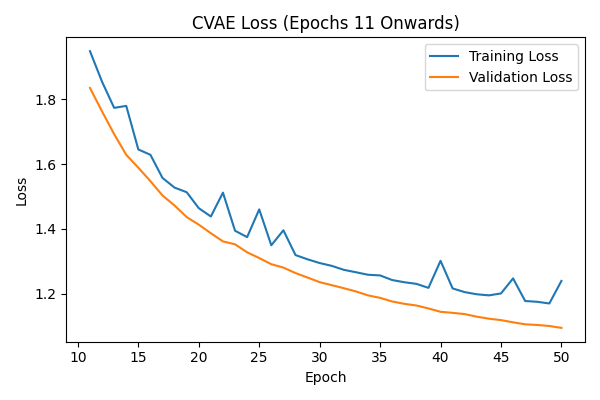
\includegraphics[width=0.7\textwidth]{cvae_lc.png}
    \caption{Learning Curve for CVAE: Training and Validation Losses over Epochs}
    \label{fig:cvae_lc}
\end{figure}

\subsection{CVAE Class Definition}

The CVAE class encapsulates the architecture of the encoder, decoder, and the reparameterization trick used in Variational Autoencoders (VAEs). Inheriting from \texttt{nn.Module}, it defines methods for encoding, reparameterizing, and decoding, thereby specifying the flow of data through the network. The encoder reduces the input dimensionality to capture latent representations, the reparameterization trick enables differentiable stochastic sampling, and the decoder reconstructs the input from the latent space conditioned on the momenta.

\subsection{Encoder Architecture}

The encoder transforms input positions into a latent space defined by a mean vector ($\mu$) and a log variance vector ($\log\sigma^2$). This is accomplished through a neural network comprising two fully connected layers with Exponential Linear Unit (ELU) activation functions that extract features from the input positions. After the second layer, the network splits into two separate branches that compute the latent mean and log variance, respectively. This design enables the model to learn a distribution over the latent variables and efficiently represent the input data in the latent space.

\subsection{Reparameterization Trick}

The reparameterization trick ensures that sampling from the latent space is differentiable, which is essential for backpropagation in gradient-based optimization. This is achieved by expressing the latent variable $\mathbf{z}$ as a deterministic function of the mean $\mu$, the standard deviation $\text{std}$, and a random variable $\epsilon$ sampled from a standard normal distribution.

The standard deviation is computed by exponentiating half of the log variance:
\begin{equation}
\text{std} = \exp\left(\frac{1}{2} \log\sigma^2\right).
\label{eq:std}
\end{equation}

A random sample $\epsilon$ is drawn from a standard normal distribution:
\begin{equation}
\epsilon \sim \mathcal{N}(0,\,I).
\label{eq:epsilon}
\end{equation}

The latent variable $\mathbf{z}$ is then calculated as:
\begin{equation}
\mathbf{z} = \mu + \epsilon \times \text{std}.
\label{eq:z}
\end{equation}

By reparameterizing $\mathbf{z}$ in this manner, the model can backpropagate gradients through the stochastic sampling process, enabling efficient training of the variational autoencoder.

\subsection{Decoder Architecture}

The decoder reconstructs the input positions from the latent variable $\mathbf{z}$, conditioned on the momenta. This is achieved by concatenating $\mathbf{z}$ with the conditioning data and processing the combined input through a neural network comprising two fully connected layers with Exponential Linear Unit (ELU) activation functions. The final output layer maps the activations back to the original input dimension, effectively reconstructing the positions.

This architecture allows the decoder to leverage both the latent representations and the conditioning information to generate accurate reconstructions. By sequentially transforming the concatenated input through the hidden layers, the decoder learns to capture the complex relationships necessary for effective reconstruction of the original positions.


\subsection{Forward Pass}

The forward pass orchestrates the flow of data through the encoder, reparameterization, and decoder, enabling the model to learn a compressed representation of the data while incorporating conditional information. It involves three main steps:

\begin{enumerate}
    \item \textbf{Encoding:} The input positions are processed by the encoder to obtain the latent mean $\mu$ and log variance $\log\sigma^2$.
    \item \textbf{Reparameterization:} A latent variable $\mathbf{z}$ is sampled using the reparameterization trick, calculated as:
    \begin{equation}
    \mathbf{z} = \mu + \epsilon \times \text{std},
    \label{eq:latent_z_forward}
    \end{equation}
    where $\epsilon \sim \mathcal{N}(0,\,I)$ and $\text{std} = \exp\left(\frac{1}{2} \log\sigma^2\right)$.
    \item \textbf{Decoding:} The latent variable $\mathbf{z}$, concatenated with the momenta, is processed by the decoder to reconstruct the input positions.
\end{enumerate}

This sequence allows the model to efficiently encode the inputs into a latent space, sample from this space in a differentiable manner, and decode the samples back into the original input space, effectively capturing the underlying data distribution conditioned on the momenta.


\subsection{Loss Function}

The loss function integrates the reconstruction loss and the Kullback-Leibler (KL) divergence to guide the training of the model effectively. The reconstruction loss encourages the model to accurately reconstruct the input positions, while the KL divergence acts as a regularizer to promote a smooth and continuous latent space.

The reconstruction loss is computed as the Mean Squared Error (MSE) between the reconstructed positions $\mathbf{\hat{x}}$ and the original input positions $\mathbf{x}$:

\begin{equation}
\mathcal{L}_{\text{recon}} = \frac{1}{n} \sum_{i=1}^{n} \left( \mathbf{x}_i - \mathbf{\hat{x}}_i \right)^2,
\label{eq:reconstruction_loss}
\end{equation}

where $n$ is the number of samples.

The KL divergence measures the difference between the learned latent distribution and the standard normal distribution, encouraging the latent variables to approximate a Gaussian distribution:

\begin{equation}
\mathcal{L}_{\text{KL}} = -\frac{1}{2} \sum_{j=1}^{d} \left( 1 + \log\sigma_j^2 - \mu_j^2 - \sigma_j^2 \right),
\label{eq:kl_divergence}
\end{equation}

where $d$ is the dimensionality of the latent space, and $\mu_j$ and $\sigma_j^2$ are the mean and variance of the $j$-th latent dimension, respectively.

The total loss is the sum of the reconstruction loss and the KL divergence:

\begin{equation}
\mathcal{L}_{\text{total}} = \mathcal{L}_{\text{recon}} + \mathcal{L}_{\text{KL}}.
\label{eq:total_loss}
\end{equation}

By minimizing $\mathcal{L}_{\text{total}}$, the model learns to reconstruct the input positions accurately while maintaining a well-structured latent space that facilitates smooth interpolation and sampling.

\subsection{Training Procedure}

The model is trained using the Adam optimizer \cite{kingma2014adam} with a learning rate of $1 \times 10^{-4}$, which provides adaptive learning rates for each parameter and accelerates the convergence of the training process. Training is conducted with a batch size of 512 to balance computational efficiency and the stability of gradient estimates.

Training is performed for up to 1000 epochs, with early stopping based on the validation loss to prevent overfitting. During each epoch, the model parameters are updated by minimizing the total loss defined in Equation~\ref{eq:total_loss}. The training and validation losses are monitored and recorded at each epoch to track the model's learning progress.

The training loop includes the following steps:

\begin{enumerate}[label=\arabic*.]
    \item \textbf{Forward Pass:} Compute the outputs of the model for the current batch.
    \item \textbf{Loss Computation:} Calculate the total loss using Equation~\ref{eq:total_loss}.
    \item \textbf{Backward Pass:} Compute gradients of the loss with respect to the model parameters.
    \item \textbf{Parameter Update:} Adjust the model parameters using the optimizer.
\end{enumerate}

The model parameters corresponding to the lowest validation loss are saved as the best model. This approach ensures that the final model generalizes well to unseen data.

\subsection{Evaluation}
\label{sec:Metrics}
After training, the model's performance is evaluated on the test dataset to assess its generalization capabilities. For each test sample, a latent vector $\mathbf{z}$ is sampled using the reparameterization trick, and the decoder reconstructs the position conditioned on the test momenta.

The evaluation metrics used to quantify the model's accuracy are:

\begin{itemize}
    \item \textbf{Mean Squared Error (MSE):} Measures the average squared difference between the predicted positions $\mathbf{\hat{x}}$ and the actual positions $\mathbf{x}$:

    \begin{equation}
    \text{MSE} = \frac{1}{n} \sum_{i=1}^{n} \left( \mathbf{x}_i - \mathbf{\hat{x}}_i \right)^2.
    \label{eq:mse}
    \end{equation}

    \item \textbf{Mean Relative Error (MRE):} Calculates the average relative difference between the predicted and actual positions, providing a normalized measure of error:

    \begin{equation}
    \text{MRE} = \frac{1}{n} \sum_{i=1}^{n} \frac{ \left| \mathbf{x}_i - \mathbf{\hat{x}}_i \right| }{ \left| \mathbf{x}_i \right| }.
    \label{eq:mre}
    \end{equation}

    The relative error is computed for each of the nine position components, and the average provides a comprehensive measure of the model's accuracy across all dimensions.
\end{itemize}

The corresponding learning curve illustrated in Figure~\ref{fig:cvae_lc}.

\begin{figure}[H]
    \centering
    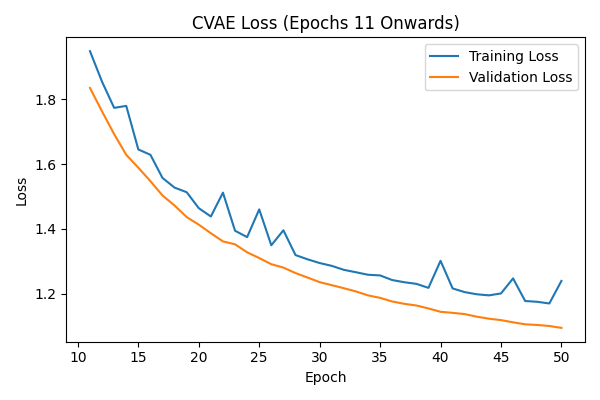
\includegraphics[width=0.7\textwidth]{cvae_lc.png}
    \caption{Learning Curve for CVAE: Training and Validation Losses over Epochs}
    \label{fig:cvae_lc}
\end{figure}

The results obtained on the test set are as follows:

\begin{itemize}
    \item \textbf{Test Mean Squared Error (MSE):} 0.6760
    \item \textbf{Mean Relative Error (MRE):} 0.7920
\end{itemize}

These metrics indicate the model's effectiveness in reconstructing the input positions from the latent space, demonstrating its ability to generalize to unseen data and capture the underlying distribution conditioned on the momenta.

\subsubsection{Ensuring No Data Leakage During Inference}
\label{subsec:Leakage}
To prevent data leakage and maintain the integrity of the model's evaluation, the CVAE strictly uses the latent representations learned from the training data during inference on the test data. During the testing phase, the model does not encode the test positions to obtain latent variables. Instead, it generates latent variables by sampling from the latent distribution parameters (mean and standard deviation) that were computed from the training latent space. The decoder then uses these sampled latent variables along with the test momenta to predict the positions. This method ensures that the test positions are not utilized at any point during inference, thereby preventing data leakage.


\subsection{Conclusion}

The CVAE model effectively captures the complex relationship between atomic positions and momenta in the dataset. By integrating conditional information and employing a structured latent space, the model achieves accurate reconstructions and demonstrates strong generalization to unseen data. The careful design of the encoder, decoder, and loss function, along with the use of the reparameterization trick, ensures that the model is both expressive and tractable during training and inference.


\section{Conditional Invertible Neural Network (cINN)}

\subsection{Overview}
The Conditional Invertible Neural Network (cINN) models the conditional distribution $p(x \mid y)$, where $x$ represents positions and $y$ represents momenta. The cINN architecture allows for efficient inference in inverse problems by mapping complex data distributions to simpler ones and vice versa through a series of invertible transformations.

\subsection{Dataset Explanation, Splitting and Model Loss Monitoring}
The methodology for preparing and monitoring our data is thoroughly discussed in subsection~\ref{subsec:Explanation}, where we explain the dataset characteristics in detail. Furthermore, the data splitting strategy and loss monitoring process described in subsection~\ref{subsec:Splitting} played a crucial role in ensuring the model's optimal performance during training.

\subsection{Overview of the cINN Architecture}
The cINN is composed of:

\begin{itemize}
    \item \textbf{Affine Coupling Layers:} Perform invertible transformations on subsets of the input.
    \item \textbf{Flip Layers:} Rearrange the order of features to ensure all dimensions are transformed.
    \item \textbf{Scale and Translate Networks:} Neural networks that compute scaling and translation factors.
    \item \textbf{cINN Model:} Assembles the layers into a complete invertible network.
\end{itemize}
These components work together to create an invertible mapping between the input data and a latent space, conditioned on additional variables.

\subsection{Affine Coupling Layer}

The Affine Coupling Layer is a fundamental component of the conditional Invertible Neural Network (cINN). It performs an invertible transformation on a subset of the input data while leaving the remaining data unchanged. This design allows for efficient computation of the Jacobian determinant, which is essential for training invertible models due to its role in the change of variables formula for probability densities.

In this layer, the input vector $\mathbf{x}$ is partitioned into two subsets, $\mathbf{x}_1$ and $\mathbf{x}_2$. For inputs with an odd number of dimensions, the division is adjusted to ensure an appropriate split between the two subsets. The transformation is applied to $\mathbf{x}_2$ using scaling and translation functions derived from $\mathbf{x}_1$ and the conditioning data $\mathbf{y}$.

The scale and translate networks take the concatenated vector $[\mathbf{x}_1,\, \mathbf{y}]$ as input and produce the scaling factors $\mathbf{s}$ and translation factors $\mathbf{t}$:

\begin{equation}
\mathbf{s},\, \mathbf{t} = \text{NN}([\mathbf{x}_1,\, \mathbf{y}]),
\label{eq:scale_translate}
\end{equation}

where $\text{NN}$ denotes a neural network.

The transformation of $\mathbf{x}_2$ is then performed using the affine coupling function:

\begin{equation}
\mathbf{x}'_2 = \mathbf{x}_2 \odot \exp(\mathbf{s}) + \mathbf{t},
\label{eq:affine_transformation}
\end{equation}

where $\odot$ represents element-wise multiplication, and $\exp(\mathbf{s})$ ensures that the scaling is strictly positive, maintaining invertibility.

The inverse transformation required for reconstructing $\mathbf{x}_2$ from $\mathbf{x}'_2$ is straightforward:

\begin{equation}
\mathbf{x}_2 = (\mathbf{x}'_2 - \mathbf{t}) \odot \exp(-\mathbf{s}).
\label{eq:inverse_affine_transformation}
\end{equation}

This invertibility is crucial for computing the exact log-likelihood during training.

By only transforming a portion of the input data at each layer, the Jacobian determinant simplifies significantly. Specifically, the determinant of the Jacobian matrix $\mathbf{J}$ for the affine coupling layer is given by:

\begin{equation}
\det(\mathbf{J}) = \exp\left( \sum_{i} s_i \right),
\label{eq:jacobian_determinant}
\end{equation}

where $s_i$ are the elements of the scaling vector $\mathbf{s}$. This expression allows for efficient computation of the log-determinant, which is necessary for the likelihood term in the loss function.

Overall, the affine coupling layer enables the cINN to model complex, invertible transformations while maintaining computational efficiency. By leveraging the conditioning data and ensuring that only a subset of the input is transformed at each layer, the model achieves a balance between expressiveness and tractability, which is essential for effective training and inference in invertible neural networks.

\subsection{Flip Layer}

The Flip Layer is integrated into the network architecture to enhance the model's expressiveness by ensuring that all elements of the input data are eventually transformed by the affine coupling layers. Specifically, after each affine coupling layer, the Flip Layer reverses the order of the elements in the input tensor along the feature dimension. This operation allows different subsets of the data to be transformed in subsequent layers, guaranteeing that all dimensions are affected by the transformations throughout the network.

By interleaving affine coupling layers with flip layers, the model overcomes the limitation where only a portion of the input is transformed in any single affine coupling layer. The flip operation ensures that the dimensions left unchanged in one layer are transformed in the next, promoting a more uniform and comprehensive transformation across all dimensions. This strategy contributes to the overall flexibility and capacity of the network, enabling it to model more complex data distributions effectively.

\subsection{Conditional Invertible Neural Network (cINN) Model}

The Conditional Invertible Neural Network (cINN) model is constructed by integrating affine coupling layers and flip layers into a comprehensive invertible architecture. This design enables the modeling of complex dependencies between atomic positions and momenta within the dataset. Specifically, the cINN comprises 20 affine coupling layers, each immediately followed by a flip layer. Both the input and condition dimensions are set to 9, corresponding to the nine-dimensional vectors representing atomic positions and momenta, respectively. The stacking of multiple affine coupling layers interleaved with flip layers allows the network to learn intricate transformations, effectively capturing the dependencies inherent in the data while ensuring that all input dimensions are transformed throughout the network.

\subsection{Scale and Translate Networks}

Within each affine coupling layer, the scale and translate networks are responsible for computing the scaling ($\mathbf{s}$) and translation ($\mathbf{t}$) factors used to transform subsets of the input data. These networks learn appropriate scaling and shifting based on the untransformed subset of the input and the conditioning information. By doing so, they enable the affine coupling layers to perform complex, data-dependent transformations while maintaining the invertibility of the overall network.

By effectively learning how to scale and shift the transformed subset of the data, the scale and translate networks play a crucial role in capturing the underlying data distribution and modeling the conditional relationships between positions and momenta. This mechanism ensures that the network can adaptively modify the transformation of input data in response to different conditioning variables, enhancing the model's expressiveness and flexibility without compromising invertibility.

\subsection{Training Procedure}

The cINN model is trained to minimize the negative log-likelihood of the data, employing optimization techniques that promote efficient convergence and generalization. The training process encompasses several key components:

\begin{itemize}
    \item \textbf{Optimization Algorithm}: An adaptive optimizer is utilized to adjust the model parameters effectively during training.
    \item \textbf{Mini-Batch Training}: The model is trained using mini-batches to balance computational efficiency with the stability of gradient estimates.
    \item \textbf{Early Stopping}: Training is monitored using validation loss to prevent overfitting, with early stopping implemented when improvements plateau.
    \item \textbf{Training Loop}:
    \begin{itemize}
        \item In each epoch, the model processes batches of data, aiming to minimize the negative log-likelihood loss function.
        \item The forward pass computes the latent representations and the log-determinant of the Jacobian, essential for calculating the loss.
        \item The loss function integrates the negative log-likelihood of the latent variables and the log-determinant of the Jacobian:
        \begin{equation}
        \mathcal{L} = -\log p(\mathbf{z}) + \log \left| \det \left( \frac{\partial \mathbf{z}}{\partial \mathbf{x}} \right) \right|,
        \label{eq:cinn_loss}
        \end{equation}
        where $p(\mathbf{z})$ denotes the probability density of the latent variables, typically assumed to follow a standard normal distribution.
        \item Gradients are computed via backpropagation, and model parameters are updated accordingly.
        \item Training and validation losses are continuously monitored to assess performance and convergence.
    \end{itemize}
\end{itemize}

The model parameters yielding the lowest validation loss are retained for subsequent evaluation, ensuring that the final model generalizes well to unseen data.

\subsection{Evaluation}

The model's performance is assessed on the test dataset to evaluate its generalization capabilities. The evaluation procedure is as follows:

\textbf{Procedure}:
\begin{itemize}
    \item For each sample in the test set:
    \begin{itemize}
        \item The forward pass computes the latent representation $\mathbf{z}$ and the log-determinant of the Jacobian.
        \item The inverse transformation reconstructs the positions $\mathbf{\hat{x}}$ from the latent variables and the test momenta $\mathbf{y}$.
    \end{itemize}
\end{itemize}

The evaluation metrics for the cINN model are consistent with those used for the CVAE model, as outlined in Section~\ref{sec:Metrics}. The results on the test dataset demonstrate the model's effectiveness:

\begin{itemize}
    \item \textbf{Mean Squared Error (MSE)}: 0.9483
    \item \textbf{Mean Relative Error (MRE)}: 0.8327
\end{itemize}

These metrics indicate that the cINN model accurately reconstructs the input positions and effectively captures the conditional distribution of positions given the momenta.

The learning curve of the cINN model, depicting the training and validation losses across epochs, is presented in Figure~\ref{fig:cinn_lc}.

\begin{figure}[H]
    \centering
    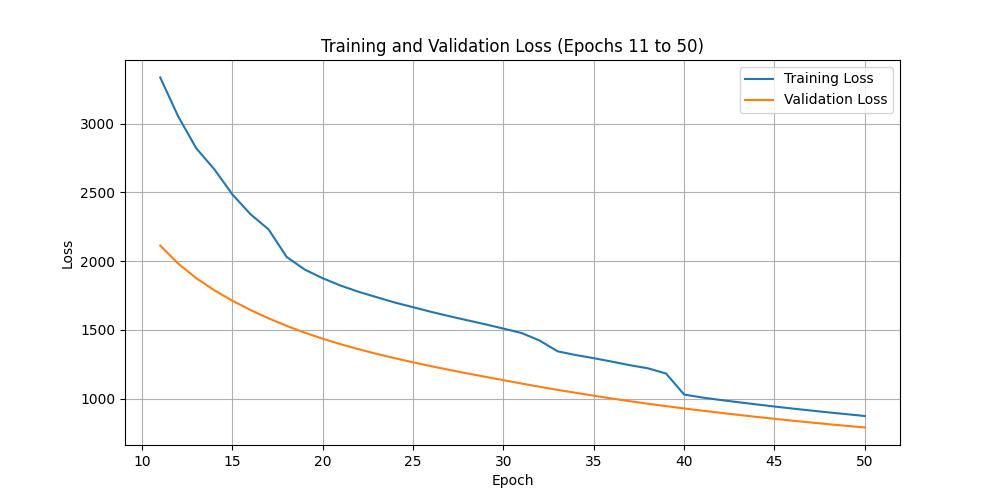
\includegraphics[width=0.7\textwidth]{cinn-lc.png}
    \caption{Learning Curve for cINN: Training and Validation Losses over Epochs}
    \label{fig:cinn_lc}
\end{figure}

These results further confirm the model's capacity to generalize to unseen data and accurately capture the conditional distribution of positions given the momenta.

\subsection{Conclusion}

The cINN model successfully models the complex relationship between atomic positions and momenta by leveraging invertible transformations and conditioning mechanisms. The integration of multiple affine coupling layers interleaved with flip layers allows the network to learn intricate mappings while maintaining computational tractability. The scale and translate networks within the affine coupling layers enable data-dependent transformations essential for capturing the underlying data distribution.

Training with the negative log-likelihood loss ensures that the model learns a probabilistic representation of the data, which is crucial for tasks such as density estimation and generative modeling. The evaluation results demonstrate that the cINN model generalizes well to unseen data, effectively reconstructing atomic positions with a high degree of accuracy.

Overall, the cINN framework presents a powerful approach for modeling conditional distributions in high-dimensional spaces, with applications extending to various domains requiring invertible and expressive neural network architectures.

\subsubsection{Ensuring No Data Leakage During Inference}

The cINN model ensures data integrity during inference by employing the same measures as described for the CVAE model in Section~\ref{subsec:Leakage}.


\end{document}
